\documentclass[14pt]{article}
\usepackage[utf8]{inputenc}
\usepackage{graphicx}
\usepackage{siunitx}
\usepackage[table]{xcolor}
\usepackage{amsmath}
\usepackage{geometry}
\geometry{a4paper,
 total={170mm,257mm},
 left=30mm,
 right=30mm,
 bottom=40mm,
 top=44mm}

\sisetup{
    group-separator={,},
    group-minimum-digits=3,
    round-mode=places,
    round-precision=2,
    table-format=3.2
}

\title{\textbf{Pump \& Motor (cc) Calculation Report}}


\date{{ doc_date | default("\\today") }}

\usepackage{eso-pic}
\AddToShipoutPictureBG{
  \AtPageUpperLeft{
    \raisebox{-\height}{
\includegraphics[width=\paperwidth]{logo.JPG}}
  }
  \AtPageLowerLeft{
    \makebox[\paperwidth]{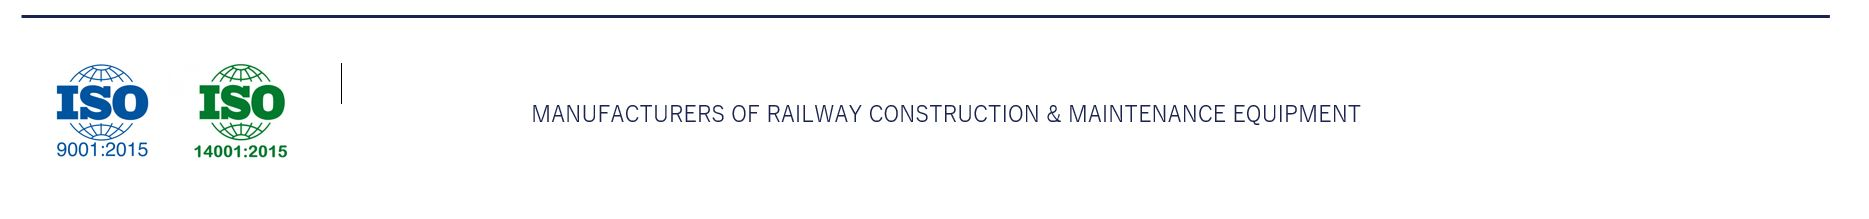
\includegraphics[height=2.3cm]{logo-1.JPG}}
  }
}

\begin{document}
\maketitle

%------------------------------------------------

\section*{\underline{Introduction}}

This document presents the theoretical analysis and calculations for determining the required hydraulic motor displacement and pump displacement for a vehicle propulsion system. The calculations evaluate wheel speed, resistance forces, torque requirements, motor performance, and hydraulic flow requirements to ensure the system meets specified operating conditions.


%------------------------------------------------

\section{\underline{Application of Theory to Vehicle}}

\subsection*{Vehicle Inputs}
\begin{itemize}
\item Vehicle Weight = {{ weight | default('N/A') }} t
\item Number of Axles = {{ axles | default('N/A') }}
\item Target Speed = {{ speed | default('N/A') }} km/h
\item Slope = {{ slope_percent | default(0) }} \%
\item Curve = {{ curve_degree | default(0) }}°
\item Wheel Diameter = {{ wheel_diameter | default('N/A') }} mm
\item PTO Ratio = {{ pto_gear_ratio | default('N/A') }}
\item Axle Ratio = {{ axle_gear_box_ratio | default('N/A') }}
\item Engine Gear Ratio = {{ engine_gear_ratio | default('N/A') }}
\item Max Vehicle RPM = {{ max_vehicle_rpm | default('N/A') }}
\end{itemize}

\subsection*{Hydraulic Inputs}
\begin{itemize}
\item Total Motors = {{ num_motors | default('N/A') }}
\item Motors per Axle = {{ per_axle_motor | default('N/A') }}
\item Total Drive Axles = {{ drive_axles | default('N/A') }}
\item Pressure = {{ pressure | default('N/A') }} bar
\item Motor Mechanical Efficiency = {{ mech_eff_motor | default('N/A') }} \%
\item Motor Volumetric Efficiency = {{ vol_eff_motor | default('N/A') }} \%
\item Pump Volumetric Efficiency = {{ vol_eff_pump | default('N/A') }} \%
\item Pump Mechanical Efficiency = {{ mech_eff_pump | default('N/A') }} \%
\item Total Pumps = {{ num_pumps | default('N/A') }}
\end{itemize}

%------------------------------------------------

\section{\underline{Calculation Procedure}}

\noindent\textbf{2 Engineering calculations}
\subsection*{2.1 Vehicle speed conversion}
\[ V = \frac{V_{km/h}}{3.6} = \frac{ {{ speed | default(0) }} }{3.6} = {{ speed_mps | default(0) | round(2) }}\;\mathrm{m/s} \]

\subsection*{2.2 Wheel circumference}
\[ D = \frac{ {{ wheel_diameter | default(0) }} }{1000} = {{ ((wheel_diameter | default(0))/1000) | round(3) }}\;\mathrm{m} \]
\[ C = \pi D = \pi \times {{ ((wheel_diameter | default(0))/1000) | round(3) }} = {{ wheel_circumference | default(0) | round(3) }}\;\mathrm{m} \]

\subsection*{2.3 Wheel rotational speed}
\[ RPM_{wheel} = \frac{V}{C} \times 60 = \frac{ {{ speed_mps | default(0) | round(2) }} }{ {{ wheel_circumference | default(0) | round(3) }} } \times 60 = {{ wheel_rpm | default(0) | round(2) }}\;\mathrm{RPM} \]

\subsection*{2.4 Gearbox input speed}
\[ RPM_{gearbox} = RPM_{wheel}\times AxleRatio = {{ wheel_rpm | default(0) | round(2) }} \times {{ axle_gear_box_ratio | default(1) }} = {{ gearbox_input_rpm | default(0) | round(2) }}\;\mathrm{RPM} \]

\subsection*{2.5 Rolling resistance (empirical)}
Empirical coefficients used: $A={{ A | default(0) | round(4) }},\; B={{ B | default(0) | round(5) }},\; C={{ C | default(0) | round(6) }}$.
\[ F_{rolling} = (A + B V + C V^{2})\times\frac{Wg}{1000} = {{ rolling_resistance | default(0) | round(2) }}\;\mathrm{kN} \]

\subsection*{2.6 Slope resistance}
\[ F_{slope} = W \times g \times \sin(\arctan(slope\%/100)) / 1000 = {{ gradient_resistance | default(0) | round(2) }}\;\mathrm{kN} \]

\subsection*{2.7 Curve resistance}
\[ F_{curve} = W \times g \times \frac{curve\_degree}{100} / 1000 = {{ curvature_resistance | default(0) | round(2) }}\;\mathrm{kN} \]

\subsection*{2.8 Starting resistance}
\[ F_{starting} = 6\times W \times \frac{g}{1000} = {{ starting_resistance | default(0) | round(2) }}\;\mathrm{kN} \]

\subsection*{2.9 Total resistance}
\[ F_{total} = F_{rolling} + F_{slope} + F_{curve} + F_{starting} = {{ total_resistance | default(0) | round(2) }}\;\mathrm{kN} \]

\subsection*{2.10 Wheel torque requirement}
Wheel radius: $r = D/2 = {{ wheel_radius | default(0) | round(3) }}\;\mathrm{m}$. 
\[ T = F_{total}\times r = {{ total_resistance | default(0) | round(2) }}\;\mathrm{kN} \times {{ wheel_radius | default(0) | round(3) }}\;\mathrm{m} = {{ required_total_torque | default(0) | round(2) }}\;\mathrm{Nm} \]

\subsection*{2.11 Torque distribution}
\[ T_{motor} = \frac{T_{total}}{N_{motors}} = \frac{{ required_total_torque | default(0) | round(2) }}{{ num_motors }} = {{ per_motor_torque | default(0) | round(2) }}\;\mathrm{Nm} \]

\subsection*{2.12 Unit conversions (examples)}
\[ T_{gearbox\_in}\; (kg\cdot cm) = {{ per_gearbox_input_torque_kg_cm | default(0) | round(2) }}\;\mathrm{kg\cdot cm} \]
\[ P\; (kg/cm^{2}) = P_{bar} \times 1.01972 = {{ pressure | default(0) }}\;\mathrm{bar} \times 1.01972 = {{ pressure_kg_cm2 | default(0) | round(2) }}\;\mathrm{kg/cm^{2}} \]

\subsection*{2.13 Motor displacement}
\[ D\; (cc/rev) = \frac{T_{(kg\cdot cm)} \times 2\pi}{P_{(kg/cm^{2})} \times \eta_{mech}} = \frac{ {{ per_gearbox_input_torque_kg_cm | default(0) | round(2) }} \times 2\pi }{ {{ pressure_kg_cm2 | default(0) | round(2) }} \times ({{ mech_eff_motor | default(0) }} / 100) } = {{ motor_displacement_cc | default(0) | round(2) }}\;\mathrm{cc/rev} \]

\subsection*{2.14 Motor flow requirement}
\[ Q_{motor} = \frac{D\times RPM_{motor}}{\eta_v\times1000} = \frac{ {{ motor_displacement_cc | default(0) | round(2) }} \times {{ max_motor_rpm | default(0) }} }{ ({{ vol_eff_motor | default(0) }} / 100) \times 1000 } = {{ per_motor_flow_rate_lpm | default(0) | round(2) }}\;\mathrm{LPM} \]
\[ Q_{total} = Q_{motor} \times {{ num_motors }} = {{ total_motor_flow_lpm | default(0) | round(2) }}\;\mathrm{LPM} \]

\subsection*{2.15 Motor power}
Hydraulic power (per motor):
\[ P_{hydraulic} = \frac{pressure_{bar}\times Q_{motor}}{600} = {{ ((pressure|default(0)) * (per_motor_flow_rate_lpm|default(0)) / 600) | round(2) }}\;\mathrm{kW} \]
Shaft output (accounting for mech. and vol. efficiency):
\[ P_{shaft} = {{ per_motor_power_kw | default(0) | round(2) }}\;\mathrm{kW} \]

\subsection*{2.16 Pump speed}
\[ RPM_{pump} = \frac{max\_vehicle\_rpm}{engine\_gear\_ratio} \times PTO\_ratio = \frac{ {{ max_vehicle_rpm | default(0) }} }{ {{ engine_gear_ratio | default(1) }} } \times {{ pto_gear_ratio | default(1) }} = {{ pump_rpm | default(0) | round(2) }}\;\mathrm{RPM} \]

\subsection*{2.17 Pump displacement}
Total pump displacement required:
\[ Pump_{total\_cc} = \frac{Q_{total}(LPM)\times1000}{RPM_{pump}\times\eta_p} = \frac{ {{ total_motor_flow_lpm | default(0) | round(2) }} \times 1000 }{ {{ pump_rpm | default(0) | round(2) }} \times ({{ vol_eff_pump | default(0) }} / 100) } = {{ pump_total_disp_cc | default(0) | round(2) }}\;\mathrm{cc/rev} \]
Per pump ({{ (pump_results[0].num_pumps if pump_results else 1) }}) :
\[ Pump_{per} = {{ (pump_results[0].pump_disp_per_pump_cc if pump_results else 0) | round(2) }}\;\mathrm{cc/rev} \]

\subsection*{2.18 Pump power}
Per-pump hydraulic power:
\[ P_{pump\_per} = {{ (pump_results[0].pump_power_per_pump_kw if pump_results else 0) | round(2) }}\;\mathrm{kW} \]

\vspace{3mm}
\noindent\textbf{3. Component selection}
\begin{tabular}{lrr}
\hline
Component & Calculated & Selected (standard) \\
\hline
Motor (cc/rev) & {{ motor_displacement_cc | default(0) | round(2) }} & {% if suggested_motor_cc %}{{ suggested_motor_cc | round(0) }}{% else %}-{% endif %} \\
Pump (per pump cc/rev) & {{ (pump_results[0].pump_disp_per_pump_cc if pump_results else 0) | round(2) }} & {% if pump_results and pump_results[0].suggested_pump_disp_per_pump_cc %}{{ pump_results[0].suggested_pump_disp_per_pump_cc | round(0) }}{% else %}-{% endif %} \\
\hline
\end{tabular}


\subsection*{Appendix: pump-results trace (summary table)}
\begin{center}
\small
\setlength{\tabcolsep}{6pt}
\begin{tabular}{l r r r r}
\hline
Engine gear & Pump RPM & Per-pump (cc) & Per-pump flow (LPM) & Per-pump P (kW) \\
\hline
{% if pump_results %}
  {% for pr in pump_results %}
    {{ pr.engine_gear_ratio }}  & {{ pr.pump_rpm | default(0) | round(2) }} & {{ pr.pump_disp_per_pump_cc | default(0) | round(2) }} & {{ pr.pump_flow_per_pump_lpm | default(0) | round(2) }} & {{ pr.pump_power_per_pump_kw | default(0) | round(2) }} \\
  {% endfor %}
\hline
{% else %}
  \multicolumn{5}{c}{No pump-result trace available.} \\
\hline
{% endif %}
\end{tabular}
\end{center}


%------------------------------------------------

\section{\underline{Summary}}

\begin{tabular}{l r}
\hline
Parameter & Value \\
\hline
Motor displacement (cc/rev) & {{ motor_displacement_cc | default(0) | round(2) }} \\
Each motor flow (LPM) & {{ per_motor_flow_rate_lpm | default(0) | round(2) }} \\
Total motor flow (LPM) & {{ total_motor_flow_lpm | default(0) | round(2) }} \\
Pump displacement per pump (cc/rev) & {{ (pump_results[0].pump_disp_per_pump_cc if pump_results else 0) | round(2) }} \\
Suggested pump displacement (cc/rev) & {{ (pump_results[0].suggested_pump_disp_per_pump_cc if pump_results else 0) | round(2) }} \\
Pump Power (total) (kW) & {{ (pump_results[0].pump_total_power_kw if pump_results else 0) | round(2) }} \\
\hline
\end{tabular}



\end{document}
